\section{Neural network settings}\label{ap:NNset}
\begin{table}[h]
	\centering
	\caption{Parameters of the compared architectures.\label{tab:architectures}}
	\footnotesize
	\begin{tabular}{|l|l|l|l|l|l|}
		\hline
		& \textbf{compact}                                                  & \textbf{compact classifier}                                       & \textbf{\begin{tabular}[c]{@{}l@{}}compact classifier\\  dilated\end{tabular}}                             & \textbf{\begin{tabular}[c]{@{}l@{}}compact classifier\\  dilated + concat\end{tabular}} & \textbf{\begin{tabular}[c]{@{}l@{}}vgg16 \\ + classifier\end{tabular}} \\ \hline \hline
		\multicolumn{6}{|l|}{\textbf{dataset parameters}} \\ \hline
		\textit{Color space}               &   YCbCr and CIELab           &   CIELab        &        CIELab                      &         CIELab                       &     CIELab                                      \\ \hline
		\textit{Fruit dataset}             & Yes                                                               & Yes                                                               & Yes                                                               & Yes                                                                                      & Yes                                                                            \\ \hline
		\textit{Landscape dataset}         & Yes                                                               & No                                                                & No                                                                & No                                                                                       & No                                                                             \\ \hline \hline
		\multicolumn{6}{|l|}{\textbf{Hyperparameter}} \\ \hline 
		\textit{Training method}           & \begin{tabular}[c]{@{}l@{}}ADADELTA\\  with momentum\end{tabular} & \begin{tabular}[c]{@{}l@{}}ADADELTA\\  with momentum\end{tabular} & \begin{tabular}[c]{@{}l@{}}ADADELTA\\  with momentum\end{tabular} & \begin{tabular}[c]{@{}l@{}}ADADELTA with \\ momentum\end{tabular}                        & \begin{tabular}[c]{@{}l@{}}ADADELTA\\  with momentum\end{tabular}              \\ \hline
		\textit{Epochs trained}            &     50       &     28  &     30   &     30                                                                                     &      25                                                                          \\ \hline
		\textit{Batch size}                &         20                                                          &     20                                                              &       20                                                            &        20                                                                                  &   20                                                                            \\ \hline \hline
		\multicolumn{6}{|l|}{\textbf{Architecture properties}} \\ \hline 
		\textit{Front end module}          & trained from scratch                                              & trained from scratch                                              & trained from scratch                                              & trained from scratch                                                                     & VGG16 front end                                                                \\ \hline
		\textit{Max pool}                  & Yes                                                               & Yes                                                               & No                                                                & No                                                                                       & Yes                                                                            \\ \hline
		\textit{Strides}                   & No                                                                & No                                                                & Yes                                                               & Yes                                                                                      & No                                                                             \\ \hline
		\textit{dilation}                  & No                                                                & No                                                                & Yes                                                               & Yes                                                                                      & No                                                                             \\ \hline
		\textit{Concatenation}             & Yes                                                               & Yes                                                               & No                                                                & Yes                                                                                      & Yes                                                                            \\ \hline
		\textit{Kernel size}               & 3x3                                                               & 3x3                                                               & 3x3                                                               & 3x3                                                                                      & 3x3                                                                            \\ \hline
		\textit{Activation function}       & ReLu                                                              & ReLu                                                              & ReLu                                                              & ReLu                                                                                     & ReLu                                                                           \\ \hline
		\textit{Batch norm}                & Yes                                                               & Yes                                                               & Yes                                                               & Yes                                                                                      & Yes                                                                            \\ \hline \hline
		\multicolumn{6}{|l|}{\textbf{Classification properties}} \\ \hline  
		\textit{Annealed mean temperature} & 0.4                                                                   &0.4                                                                   &0.4                                                                   &0.4                                                                                          &0.4                                                                                \\ \hline
		\textit{K-nearest neighbour}       & -                                                                 & 10                                                                & 10                                                                & 10                                                                                       & 10                                                                             \\ \hline
		\textit{K-nearest neighbour sigma} & -                                                                 & 5                                                                 & 5                                                                 & 5                                                                                        & 5                                                                              \\ \hline
		\textit{Number of colorbins} & -                                                                 & 247                                                                 & 247                                                                 & 247                                                                                        & 247                                                                              \\ \hline
		\textit{Uniform mixing factor ($\lambda$)} & -                                                                 & 0.3                                                                 & 0.3                                                                 & 0.3                                                                                        & 0.5                                                                              \\ \hline
	\end{tabular}
\end{table}

\newpage
\section{More results}\label{ap:more_results}
\begin{figure}[h]
	\centering
	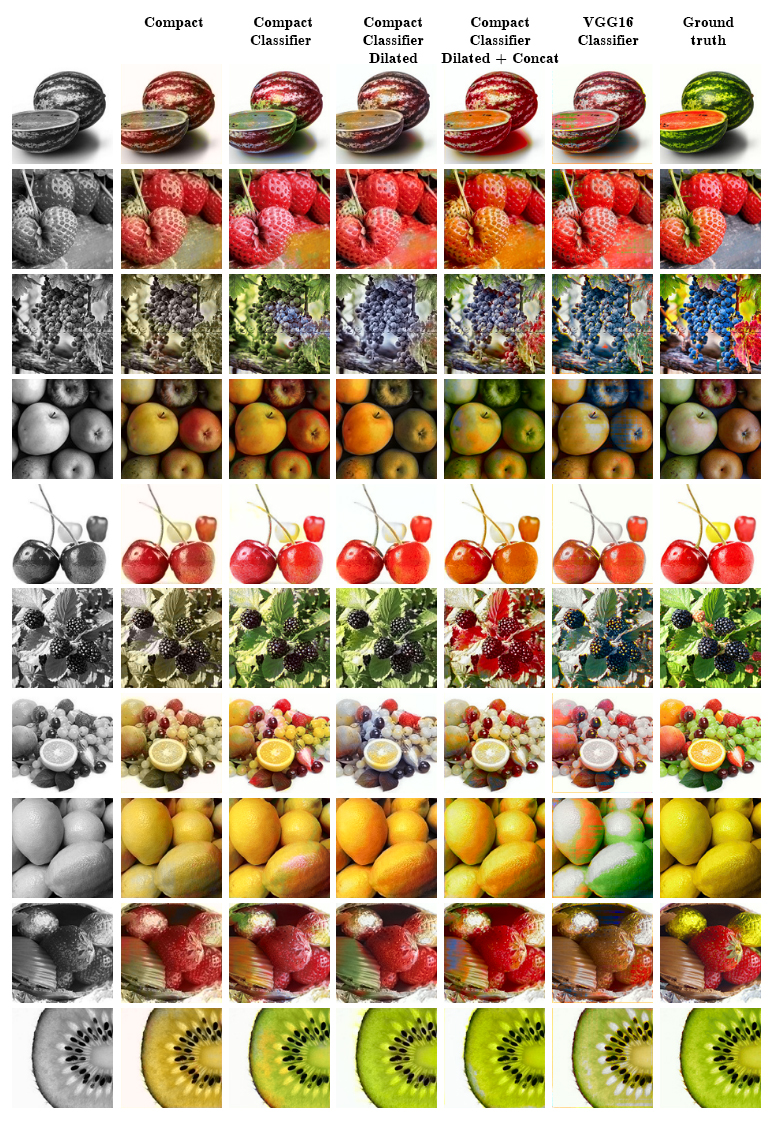
\includegraphics[width=0.83\textwidth]{set1}
	\label{fig:moreresults}
\end{figure}

\newpage
%%error plots here




\section{Training and validation errors}\label{ap:errors}

\begin{figure}[h]
	\centering
	\begin{subfigure}[b]{0.45\textwidth}
		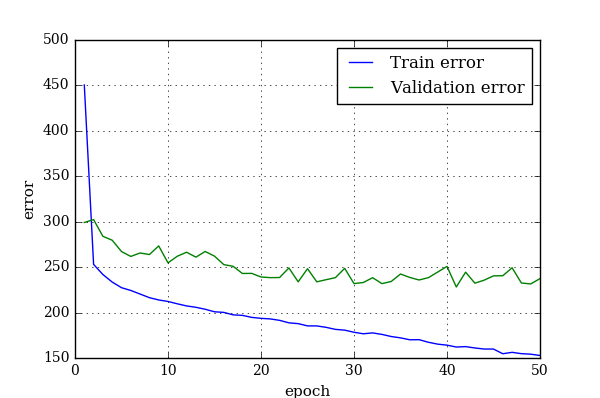
\includegraphics[width=\textwidth]{errors_fruit_Compact_more_end_fmaps_YCbCr_sigma3}
		\caption{Compact}
		\label{fig:eror_comp_class}
	\end{subfigure}
	\begin{subfigure}[b]{0.45\textwidth}
		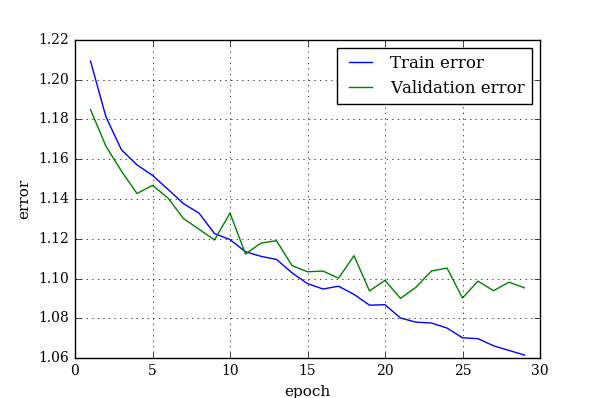
\includegraphics[width=\textwidth]{errors_fruit_Compact_more_end_fmaps_classifier_k10_T02_sigma5_nbins20_labda_03_gridsize10}
		\caption{Compact classifier}
		\label{fig:eror_comp_class}
	\end{subfigure}
	~ %add desired spacing between images, e. g. ~, \quad, \qquad, \hfill etc. 
	%(or a blank line to force the subfigure onto a new line)
	\begin{subfigure}[b]{0.45\textwidth}
		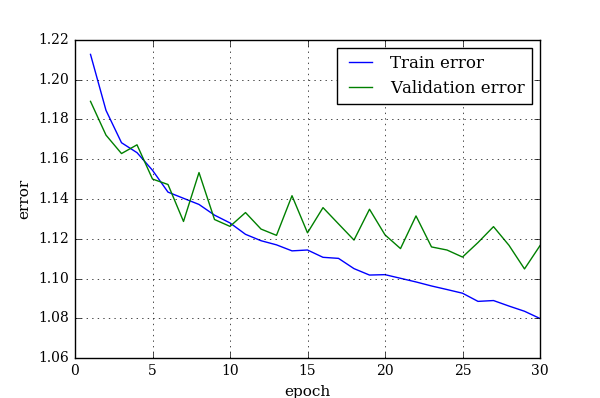
\includegraphics[width=\textwidth]{errors_fruit_Compact_more_end_fmaps_dilation_concat_k10_T02_sigma5_nbins20_labda_03_gridsize10.png}
		\caption{Compact classifier dilation + concat}
		\label{fig:error_comp_class_dila_con}
	\end{subfigure}
	~ %add desired spacing between images, e. g. ~, \quad, \qquad, \hfill etc. 
	%(or a blank line to force the subfigure onto a new line)
	\begin{subfigure}[b]{0.45\textwidth}
		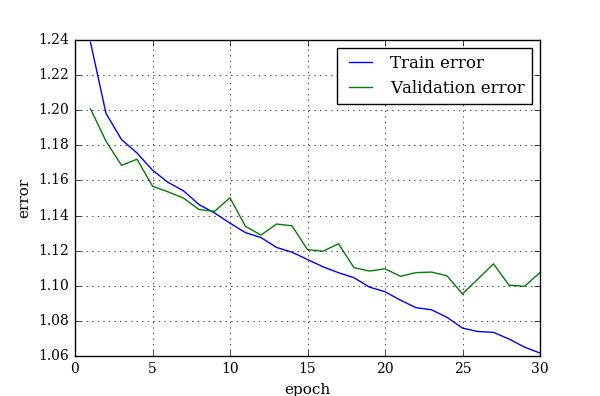
\includegraphics[width=\textwidth]{errors_fruit_Compact_more_end_fmaps_dilation_k10_T02_sigma5_nbins20_labda_03_gridsize10}
		\caption{Compact classifier dilation}
		\label{fig:error_comp_class_dila}
	\end{subfigure}
	\caption{The error plots for the different architectures. Note the large difference between the validation error and the train error for the compact architecture. That is due to the blur that is applied to the train dataset but not to the validation training set.}\label{fig:animals}
\end{figure}